\clearpage

\section{Translucent without Survivability}\label{ILP_Transluc_Survivability}

\subsection{Model description}

First of all, in order to use the ILP model, we must take into account the physical and logical topologies allowed by this mode of transport and the type of survivability. Through the following figures, you can see these topologies. \\

\begin{figure}[h!]
\centering
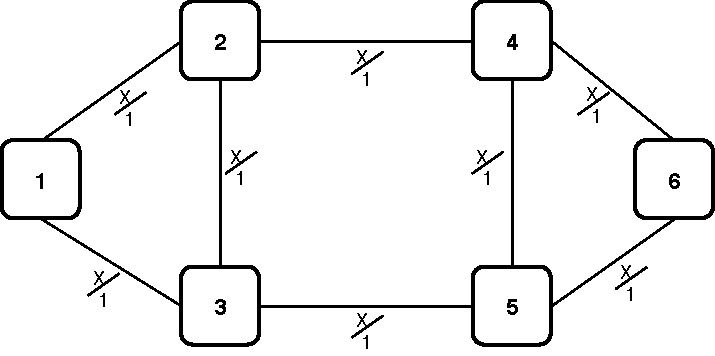
\includegraphics[width=11cm]{sdf/ilp/translucent_survivability/figures/allowed_physical_topology}
\caption{Translucent without survivability: Allowed physical topology. The allowed physical topology is defined by the duct and sites in the field. It is assumed that each duct supports up to 1 bidirectional transmission system and each site supports up to 1 node.}
\label{allowed3_physical_low}
\end{figure}

\vspace{15pt}
\begin{figure}[h!]
\centering
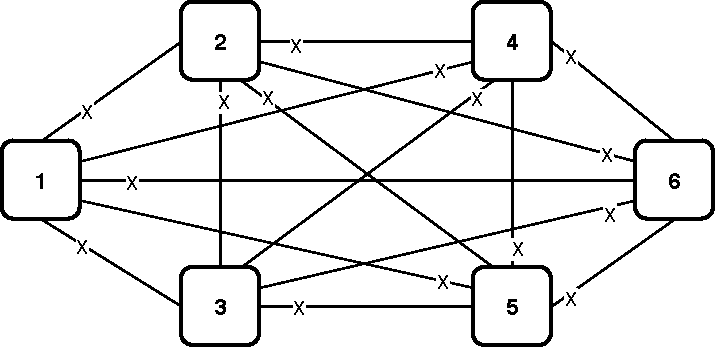
\includegraphics[width=11cm]{sdf/ilp/translucent_survivability/figures/allowed_optical_topology}
\caption{Translucent without survivability: Allowed optical topology. The allowed optical topology is defined by the transport mode. It is assumed that each connections between demands supports up to 100 lightpaths.}
\label{allowed3_optical_low}
\end{figure}

Now taking this into consideration and based on the specific constraints of the translucent mode without survivability it is possible to define the ILP model.\\
\newpage
The objective function, to be minimized, is the expression \ref{ILPOpaque_CAPEX}, i.e.,
\begin{equation*}
  minimize \qquad \Big\{ \quad C_C \quad \Big\}
\end{equation*}

$subject$ $to$
\begin{equation}
\sum_{k\textbackslash \{o\}} Ls_{pk}^{odc} = D_{odc} \qquad \qquad \qquad \qquad \qquad \qquad \qquad
\forall(o,d,c) : o < d, \forall p: p = o
\label{ILPTransluc1}
\end{equation}
\noindent
This are the virtual flow conservation constraints and ensure that, for each $(o,d)$ pair, we route client demand units of flow from node $o$ to node $d$, the source node sends client demand units of flow.

\begin{equation}
\sum_{k\textbackslash \{p,o\}} Ls_{pk}^{odc} = \sum_{k\textbackslash \{p,d\}} Ls_{kp}^{odc} \qquad \qquad \qquad \qquad
\forall(o,d,c) : o < d, \forall p: p \neq o,d
\label{ILPTransluc2}
\end{equation}
\noindent
This constraint ensure that the remaining nodes, being neither origin or destination, the receive flow have to be send.

\begin{equation}
\sum_{k\textbackslash \{d\}} Ls_{kp}^{odc} = D_{odc} \qquad \qquad \qquad \qquad \qquad \qquad \qquad \qquad
\forall(o,d,c) : o < d, \forall p: p = d
\label{ILPTransluc3}
\end{equation}
\noindent
This are the virtual flow conservation constraints and ensure that, for each $(o,d)$ pair, we route client demand units of flow from node $o$ to node $d$, the destination node has to receive those client demand units of flow.

\begin{equation}
\sum_{o=1} \sum_{d=o+1} B(c)(Ls_{pk}^{odc} + Ls_{kp}^{odc}) \leq  \tau \lambda_{pk} \qquad \qquad \qquad \qquad \qquad \qquad
\forall (p,k) : p < k, \forall c
\label{ILPTransluc4}
\end{equation}
\noindent
This restriction is considered grooming constraint and the variable $\tau$ is always 100 Gbits/s.

\begin{equation}
\sum_{j\textbackslash \{p\}} f_{ij}^{pk} = \lambda_{pk}  \qquad \qquad \qquad \qquad \qquad \qquad \qquad \qquad \qquad
\forall(p,k) : p < k, \forall i: i = p
\label{ILPTransluc6}
\end{equation}
\noindent
This constraint are equal to the constraint \ref{ILPOpaque1_CAPEX} assuming that Z variable has the value of number of optical channels between this demand for all bidirectional links.

\begin{equation}
\sum_{j\textbackslash \{p\}} f_{ij}^{pk} = \sum_{j\textbackslash \{k\}} f_{ji}^{pk} \qquad \qquad \qquad \qquad \qquad \qquad \qquad \qquad
\forall(p,k) : p < k, \forall i: i \neq p,k
\label{ILPTransluc7}
\end{equation}
\noindent
This constraint are equal to the constraint \ref{ILPOpaque2_CAPEX}.

\begin{equation}
\sum_{j\textbackslash \{k\}} f_{ji}^{pk} = \lambda_{pk}  \qquad \qquad \qquad \qquad \qquad \qquad \qquad \qquad \qquad
\forall(p,k) : p < k, \forall i: i = k
\label{ILPTransluc8}
\end{equation}
\noindent
This constraint are equal to the constraint \ref{ILPOpaque3_CAPEX} assuming that Z variable has the value of number of optical channels between this demand for all bidirectional links.

\begin{equation}
\sum_{p=1} \sum_{k=p+1} \left( f_{ij}^{pk} + f_{ji}^{pk}\right) \leq K_{ij} G_{ij} L_{ij} \qquad \qquad \qquad \qquad \qquad \qquad \qquad
\forall (i,j) : i < j
\label{ILPTransluc9}
\end{equation}
\noindent
This restriction answers capacity constraint problem. Then, total flows must be less or equal to the capacity of network links. For any situation the maximum number of optical channels supported by each transmission system is 100, i.e., $K_{ij}$ = 100.

\begin{equation}
f_{ij}^{pk} , f_{ji}^{pk} , Ls_{pk}^{odc} , Ls_{kp}^{odc} , \lambda_{pk} \in \mathbb{N}   \qquad \qquad \qquad \qquad \qquad
\forall(i,j) : i < j, \forall(o,d) : o < d
\label{ILPTransluc10}
\end{equation}
\noindent
This constraint defines that these variables must be a counting number.

\begin{equation}
L_{i,j} \in \{0,1\} \qquad \qquad \qquad \qquad \qquad \qquad \qquad \qquad \qquad \qquad \qquad \qquad \qquad \qquad
\forall(i,j)
\label{ILPTransluc11}
\end{equation}
\noindent
Last constraint refers to the use of the link where this variable can be zero if it is not being used or one if is being used.

\subsection{Result description}

To perform the calculations using the implementation of the models described previously it is necessary to use once more the MATLAB. We have all the necessary to obtain the CAPEX value for the reference network \ref{Reference_Network_Topology}.\\

\textbf{Low Traffic Scenario:}\\

In this scenario we have to take into account the traffic calculated in \ref{low_scenario}. In a first phase, we will show the resulting physical and optical topology. These topologies are based on the allowed topologies referred to in the model description and also taking into account the logical topology for all ODUs mentioned in the section \ref{low_scenario}.\\

\newpage
\begin{figure}[h!]
\centering
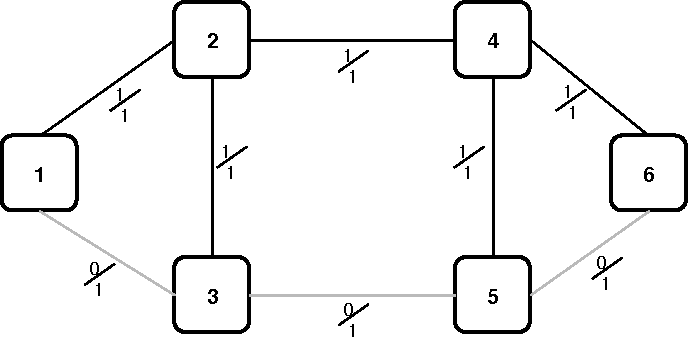
\includegraphics[width=12cm]{sdf/ilp/translucent_survivability/figures/physical_topology_low}
\caption{Translucent without survivability in low scenario: Physical topology after dimensioning.}
\label{physical3_low}
\end{figure}

\begin{figure}[h!]
\centering
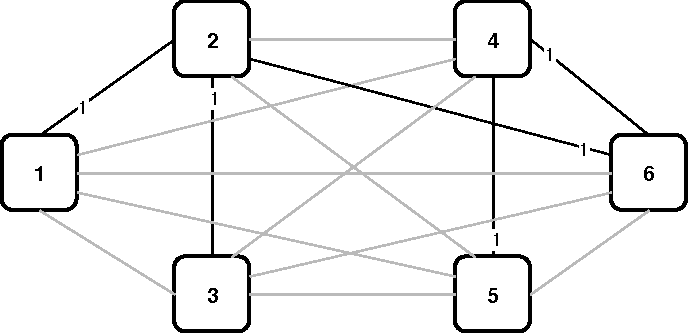
\includegraphics[width=12cm]{sdf/ilp/translucent_survivability/figures/optical_topology_low}
\caption{Translucent without survivability in low scenario: Optical topology after dimensioning.}
\label{optical3_low}
\end{figure}

In table \ref{link_transluc_surv_ref_low} we can see the number of optical channels calculated using \ref{Capex_Link} and \ref{ILPOpaque_CAPEX} and the number of amplifiers for each link calculated using \ref{Capex_amplifiers}. In the case where there are no optical channels we assume that the number of amplifiers is zero.\\

\begin{table}[h!]
\centering
\begin{tabular}{|| c | c | c ||}
 \hline
 \multicolumn{3}{|| c ||}{Information regarding links} \\
 \hline
 \hline
 Bidirectional Link & Optical Channels & Amplifiers\\
 \hline
 Node 1 <-> Node 2 & 1 & 4 \\
 Node 1 <-> Node 3 & 0 & 0 \\
 Node 2 <-> Node 3 & 1 & 0 \\
 Node 2 <-> Node 4 & 1 & 6 \\
 Node 3 <-> Node 5 & 0 & 0 \\
 Node 4 <-> Node 5 & 1 & 1 \\
 Node 4 <-> Node 6 & 2 & 7 \\
 Node 5 <-> Node 6 & 0 & 0 \\
 \hline
\end{tabular}
\caption{Table with information regarding links for translucent mode without survivability in low scenario.}
\label{link_transluc_surv_ref_low}
\end{table}

\newpage
In table \ref{node_transluc_surv_ref_low} we can see the resulting nodal degree at the physical layer, the number of line ports and add ports using \ref{OXC_poxc_transluc} the number of LR transponders using \ref{EXC_pexc2_transluc} and the number of tributary ports using \ref{EXC_pexc1_transluc}.

\begin{table}[h!]
\centering
\begin{tabular}{|| c | c | c | c | c | c ||}
 \hline
 \multicolumn{6}{|| c ||}{Information regarding nodes} \\
 \hline
 \hline
 \multicolumn{2}{|| c |}{ } & \multicolumn{2}{ c |}{Electrical part} & \multicolumn{2}{ c ||}{Optical part} \\
 \hline
 Node & Resulting Nodal Degree & Tributary Ports & LR Transponders & Add Ports & Line Ports\\
 \hline
 1 & 1 & 29 & 1 & 1 & 1 \\
 2 & 3 & 23 & 3 & 3 & 3 \\
 3 & 1 & 18 & 1 & 1 & 1 \\
 4 & 3 & 20 & 2 & 2 & 4 \\
 5 & 1 & 24 & 1 & 1 & 1 \\
 6 & 1 & 22 & 2 & 2 & 2 \\
\hline
\end{tabular}
\caption{Table with information regarding nodes for translucent mode without survivability in low scenario.}
\label{node_transluc_surv_ref_low}
\end{table}

Through the information obtained previously on the nodes we can now create tables with detailed information about each node. In each table mentioned below we can see how many ports are connected to a given node and its bit rate, the number of LR transponders and how many ports are assigned to each different bit rate.\\

\begin{table}[h!]
\centering
\begin{tabular}{|| c | c | c ||}
 \hline
 \multicolumn{3}{|| c ||}{Detailed description of Node 1} \\
 \hline
 \hline
 Electrical part & Number of total demands & Bit rate \\
 \hline
\multirow{3}{*}{29 tributary ports} & 13 & ODU0 \\
 & 13 & ODU1 \\
 & 3 & ODU2 \\
 \hline
  & Node<--Optical Channels-->Node & Bit rate \\
 \hline
 1 LR Transponders & 1  <---- 1 ---->  2 & 100 Gbits/s \\
 \hline
 \hline
 Optical part & Node<--Optical Channels-->Node & Bit rate \\
 \hline
 1 add ports & 1  <---- 1 ---->  2 & \multirow{2}{*}{100 Gbits/s} \\ \cline{1-2}
 1 line ports & 1  <---- 1 ---->  2 & \\
\hline
\end{tabular}
\caption{Translucent without survivability in low scenario: Detailed description of node 1. The number of demands is distributed to the various destination nodes, this distribution can be observed in section \ref{low_scenario}.}
\end{table}

\newpage
\begin{table}[h!]
\centering
\begin{tabular}{|| c | c | c ||}
 \hline
 \multicolumn{3}{|| c ||}{Detailed description of Node 2} \\
 \hline
 \hline
 Electrical part & Number of total demands & Bit rate \\ \hline
\multirow{5}{*}{23 tributary ports} & 11 & ODU0 \\
 & 7 & ODU1 \\
 & 2 & ODU2 \\
 & 2 & ODU3 \\
 & 1 & ODU4 \\
 \hline
  & Node<--Optical Channels-->Node & Bit rate \\
  \hline
\multirow{3}{*}{3 LR Transponders} & 2  <---- 1 ---->  1 & \multirow{3}{*}{100 Gbits/s} \\
  & 2  <---- 1 ---->  3 & \\
  & 2  <---- 1 ---->  6 & \\
 \hline
 \hline
 Optical part & Node<--Optical Channels-->Node & Bit rate \\
 \hline
 \multirow{3}{*}{3 add ports} & 2  <---- 1 ---->  1 & \multirow{6}{*}{100 Gbits/s} \\
  & 2  <---- 1 ---->  3 & \\
  & 2  <---- 1 ---->  6 & \\ \cline{1-2}
 \multirow{3}{*}{3 line ports} & 2  <---- 1 ---->  1 & \\
  & 2  <---- 1 ---->  3 & \\
  & 2  <---- 1 ---->  6 & \\
\hline
\end{tabular}
\caption{Translucent without survivability in low scenario: Detailed description of node 2. The number of demands is distributed to the various destination nodes, this distribution can be observed in section \ref{low_scenario}.}
\end{table}

\begin{table}[h!]
\centering
\begin{tabular}{|| c | c | c ||}
 \hline
 \multicolumn{3}{|| c ||}{Detailed description of Node 3} \\
 \hline
 \hline
 Electrical part & Number of total demands & Bit rate \\
 \hline
 \multirow{4}{*}{18 tributary ports} & 7 & ODU0 \\
 & 6 & ODU1\\
 & 3 & ODU2\\
 & 2 & ODU3\\
 \hline
  & Node<--Optical Channels-->Node & Bit rate \\ \hline
  1 LR Transponders & 3  <---- 1 ---->  2 & 100 Gbits/s \\
 \hline
 \hline
 Optical part & Node<--Optical Channels-->Node & Bit rate \\
 \hline
 1 add ports & 3  <---- 1 ---->  2 & \multirow{2}{*}{100 Gbits/s} \\ \cline{1-2}
 1 line ports & 3  <---- 1 ---->  2 & \\
\hline
\end{tabular}
\caption{Translucent without survivability in low scenario: Detailed description of node 3. The number of demands is distributed to the various destination nodes, this distribution can be observed in section \ref{low_scenario}.}
\end{table}

\newpage
\begin{table}[h!]
\centering
\begin{tabular}{|| c | c | c ||}
 \hline
 \multicolumn{3}{|| c ||}{Detailed description of Node 4} \\
 \hline
 \hline
 Electrical part & Number of total demands & Bit rate \\ \hline
\multirow{3}{*}{20 tributary ports} & 7 & ODU0 \\
 & 10 & ODU1 \\
 & 3 & ODU2 \\
 \hline
  & Node<--Optical Channels-->Node & Bit rate \\ \hline
 \multirow{2}{*}{2 LR Transponders} & 4  <---- 1 ---->  5 & \multirow{2}{*}{100 Gbits/s} \\
  & 4  <---- 1 ---->  6 & \\
 \hline
 \hline
 Optical part & Node<--Optical Channels-->Node & Bit rate \\
 \hline
 \multirow{2}{*}{2 add ports} & 4  <---- 1 ---->  5 & \multirow{5}{*}{100 Gbits/s} \\
  & 4  <---- 1 ---->  6 & \\ \cline{1-2}
 \multirow{3}{*}{4 line ports} & 4  <---- 1 ---->  5 & \\
  & 4  <---- 1 ---->  6 & \\
  & 2  <---- 1 ---->  6 & \\
\hline
\end{tabular}
\caption{Translucent without survivability in low scenario: Detailed description of node 4. The number of demands is distributed to the various destination nodes, this distribution can be observed in section \ref{low_scenario}. Regarding the number of line ports when this node is different to the source, it means that through ports are used. In the latter the number of ports is double the number of optical channels.}
\end{table}

\begin{table}[h!]
\centering
\begin{tabular}{|| c | c | c ||}
 \hline
 \multicolumn{3}{|| c ||}{Detailed description of Node 5} \\
 \hline
 \hline
 Electrical part & Number of total demands & Bit rate \\ \hline
\multirow{5}{*}{24 tributary ports} & 14 & ODU0 \\
 & 4 & ODU1 \\
 & 4 & ODU2 \\
 & 1 & ODU3 \\
 & 1 & ODU4 \\
 \hline
  & Node<--Optical Channels-->Node & Bit rate \\ \hline
  1 LR Transponders & 5  <---- 1 ---->  4 & 100 Gbits/s \\
 \hline
 \hline
 Optical part & Node<--Optical Channels-->Node & Bit rate \\
 \hline
 1 add ports & 5  <---- 1 ---->  4 & \multirow{2}{*}{100 Gbits/s} \\ \cline{1-2}
 1 line ports & 5  <---- 1 ---->  4 & \\
\hline
\end{tabular}
\caption{Translucent without survivability in low scenario: Detailed description of node 5. The number of demands is distributed to the various destination nodes, this distribution can be observed in section \ref{low_scenario}.}
\end{table}

\newpage
\begin{table}[h!]
\centering
\begin{tabular}{|| c | c | c ||}
 \hline
 \multicolumn{3}{|| c ||}{Detailed description of Node 6} \\
 \hline
 \hline
 Electrical part & Number of total demands & Bit rate \\ \hline
\multirow{5}{*}{22 tributary ports} & 8 & ODU0 \\
 & 10 & ODU1 \\
 & 1 & ODU2 \\
 & 1 & ODU3 \\
 & 2 & ODU4 \\
 \hline
  & Node<--Optical Channels-->Node & Bit rate \\ \hline
 \multirow{2}{*}{2 LR Transponders} & 6  <---- 1 ---->  2 & \multirow{2}{*}{100 Gbits/s} \\
  & 6  <---- 1 ---->  4 & \\
 \hline
 Optical part & Node<--Optical Channels-->Node & Bit rate \\
 \hline
 \multirow{2}{*}{2 add ports} & 6  <---- 1 ---->  2 & \multirow{4}{*}{100 Gbits/s} \\
  & 6  <---- 1 ---->  4 & \\ \cline{1-2}
 \multirow{2}{*}{2 line ports} & 6  <---- 1 ---->  2 & \\
  & 6  <---- 1 ---->  4 & \\
\hline
\end{tabular}
\caption{Translucent without survivability in low scenario: Detailed description of node 6. The number of demands is distributed to the various destination nodes, this distribution can be observed in section \ref{low_scenario}.}
\end{table}

Now, let's focus on the routing information in table \ref{path_transluc_surv_ref_low}. These paths are bidirectional so the path from one node to another is the same path in the opposite direction.\\

\begin{table}[h!]
\centering
\begin{tabular}{|| c | c | c | c ||}
 \hline
 \multicolumn{4}{|| c ||}{Routing} \\
 \hline
 \hline
 o & d & Links & Demands \\
 \hline
 1 & 2 & \{(1,2)\} & 5 ODU0, 2 ODU1, 1 ODU2 \\ \hline
 1 & 3 & \{(1,2),(2,3)\} & 1 ODU0, 4 ODU1, 1 ODU2 \\ \hline
 1 & 4 & \{(1,2),(2,4),(4,6),(6,4)\} & 3 ODU0, 2 ODU1, 1 ODU2 \\ \hline
 1 & 5 & \{(1,2),(2,4),(4,6),(6,4),(4,5)\} & 1 ODU0 \\ \hline
 1 & 6 & \{(1,2),(2,4),(4,6)\} & 3 ODU0, 5 ODU1 \\ \hline
 2 & 3 & \{(2,3)\} & 1 ODU3 \\ \hline
 2 & 4 & \{(2,4),(4,6),(6,4)\} & 1 ODU0, 3 ODU1 \\ \hline
 2 & 5 & \{(2,4),(4,6),(6,4),(4,5)\} & 5 ODU0, 1 ODU1, 1 ODU2 \\ \hline
 2 & 6 & \{(2,4),(4,6)\} & 1 ODU1, 1 ODU3, 1 ODU4 \\ \hline
 3 & 4 & \{(3,2),(2,4),(4,6),(6,4)\} & 1 ODU0, 1 ODU1, 1 ODU2 \\ \hline
 3 & 5 & \{(3,2),(2,4),(4,6),(6,4),(4,5)\} & 4 ODU0, 1 ODU1, 1 ODU2, 1 ODU3 \\ \hline
 3 & 6 & \{(3,2),(2,4),(4,6)\} & 1 ODU0 \\ \hline
 4 & 5 & \{(4,5)\} & 1 ODU0, 1 ODU1, 1 ODU2 \\ \hline
 4 & 6 & \{(4,6)\} & 1 ODU0, 3 ODU1\\ \hline
 5 & 6 & \{(5,4),(4,6)\} & 3 ODU0, 1 ODU1, 1 ODU2, 1 ODU4 \\
 \hline
\end{tabular}
\caption{Translucent without survivability in low scenario: Description of demands routing. In this case all the demands follow the same path for a certain pair of nodes, but this may not happen for other cases.}
\label{path_transluc_surv_ref_low}
\end{table}
\newpage
Lastly through table \ref{scripttransluc_surv_ref_low} we can see the CAPEX result for this model. This value is obtained using equation \ref{ILPOpaque_CAPEX} and all of the constraints mentioned above.\\

\begin{table}[h!]
\centering
\begin{tabular}{|| c | c | c | c | c | c | c ||}
 \hline
 \multicolumn{7}{|| c ||}{CAPEX of the Network} \\
 \hline
 \hline
 \multicolumn{3}{|| c |}{ } & Quantity & Unit Price & Cost & Total \\
 \hline
 \multirow{3}{*}{Link Cost} & \multicolumn{2}{ c |}{OLTs} & 10 & 15 000 \euro & 150 000 \euro & \multirow{3}{*}{6 294 000 \euro} \\ \cline{2-6}
 & \multicolumn{2}{ c |}{100 Gbits/s Transceivers} & 12 & 5 000 \euro/Gbit/s & 6 000 000 \euro & \\ \cline{2-6}
 & \multicolumn{2}{ c |}{Amplifiers} & 36 & 4 000 \euro & 144 000 \euro & \\
 \hline
 \multirow{10}{*}{Node Cost} & \multirow{7}{*}{Electrical} & EXCs & 6 & 10 000 \euro & 60 000 \euro & \multirow{10}{*}{1 237 590 \euro} \\ \cline{3-6}
 & & ODU0 Ports & 60 & 10 \euro/port & 600 \euro & \\ \cline{3-6}
 & & ODU1 Ports & 50 & 15 \euro/port & 750 \euro & \\ \cline{3-6}
 & & ODU2 Ports & 16 & 30 \euro/port & 480 \euro & \\ \cline{3-6}
 & & ODU3 Ports & 6 & 60 \euro/port & 360 \euro & \\ \cline{3-6}
 & & ODU4 Ports & 4 & 100 \euro/port & 400 \euro & \\ \cline{3-6}
 & &Transponders& 10 & 100 000 \euro/port & 1 000 000 \euro & \\ \cline{2-6}
 & \multirow{3}{*}{Optical} & OXCs & 6 & 20 000 \euro & 120 000 \euro & \\ \cline{3-6}
 & & Line Ports & 12 & 2 500 \euro/port & 30 000 \euro & \\ \cline{3-6}
 & & Add Ports & 10 & 2 500 \euro/port & 25 000 \euro & \\
 \hline
 \multicolumn{6}{|| c |}{Total Network Cost} & 7 531 590 \euro \\
\hline
\end{tabular}
\caption{Translucent without survivability in low scenario: Detailed description of CAPEX for this scenario.}
\label{scripttransluc_surv_ref_low}
\end{table}

\textbf{Medium Traffic Scenario:}\\

In this scenario we have to take into account the traffic calculated in \ref{medium_traffic_scenario}. In a first phase, we will show the resulting physical and optical topology. These topologies are based on the allowed topologies referred to in the model description and also taking into account the logical topology for all ODUs mentioned in the section \ref{medium_traffic_scenario}.\\

\begin{figure}[h!]
\centering
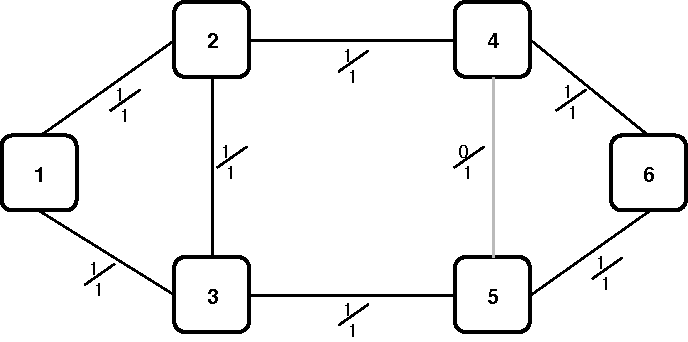
\includegraphics[width=12cm]{sdf/ilp/translucent_survivability/figures/physical_topology_medium}
\caption{Translucent without survivability in medium scenario: Physical topology after dimensioning.}
\label{physical3_medium}
\end{figure}

\newpage
\begin{figure}[h!]
\centering
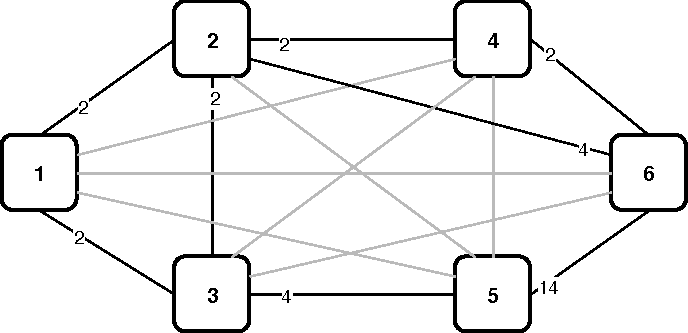
\includegraphics[width=12cm]{sdf/ilp/translucent_survivability/figures/optical_topology_medium}
\caption{Translucent without survivability in medium scenario: Optical topology after dimensioning.}
\label{optical3_medium}
\end{figure}

In table \ref{link_transluc_surv_ref_medium} we can see the number of optical channels calculated using \ref{Capex_Link} and \ref{ILPOpaque_CAPEX} and the number of amplifiers for each link calculated using \ref{Capex_amplifiers}.
In table \ref{node_transluc_surv_ref_medium} we can see the resulting nodal degree at the physical layer, the number of line ports and add ports using \ref{OXC_poxc_transluc} the number of LR transponders using \ref{EXC_pexc2_transluc} and the number of tributary ports using \ref{EXC_pexc1_transluc}.

\begin{table}[h!]
\centering
\begin{tabular}{|| c | c | c ||}
 \hline
 \multicolumn{3}{|| c ||}{Information regarding links} \\
 \hline
 \hline
 Bidirectional Link & Optical Channels & Amplifiers\\
 \hline
 Node 1 <-> Node 2 & 2 & 4 \\
 Node 1 <-> Node 3 & 2 & 6 \\
 Node 2 <-> Node 3 & 2 & 0 \\
 Node 2 <-> Node 4 & 6 & 6 \\
 Node 3 <-> Node 5 & 4 & 8 \\
 Node 4 <-> Node 5 & 0 & 0 \\
 Node 4 <-> Node 6 & 6 & 7 \\
 Node 5 <-> Node 6 & 14 & 3 \\
 \hline
\end{tabular}
\caption{Table with information regarding links for translucent mode without survivability in medium scenario.}
\label{link_transluc_surv_ref_medium}
\end{table}

\begin{table}[h!]
\centering
\begin{tabular}{|| c | c | c | c | c | c ||}
 \hline
 \multicolumn{6}{|| c ||}{Information regarding nodes} \\
 \hline
 \hline
 \multicolumn{2}{|| c |}{ } & \multicolumn{2}{ c |}{Electrical part} & \multicolumn{2}{ c ||}{Optical part} \\
 \hline
 Node & Resulting Nodal Degree & Tributary Ports & LR Transponders & Add Ports & Line Ports\\
 \hline
 1 & 2 & 290 & 4 & 4 & 4 \\
 2 & 3 & 230 & 10 & 10 & 10 \\
 3 & 3 & 180 & 8 & 8 & 8 \\
 4 & 2 & 200 & 4 & 4 & 12 \\
 5 & 2 & 240 & 18 & 18 & 18 \\
 6 & 2 & 220 & 20 & 20 & 20 \\
\hline
\end{tabular}
\caption{Table with information regarding nodes for translucent mode without survivability in medium scenario.}
\label{node_transluc_surv_ref_medium}
\end{table}

\newpage
Through the information obtained previously on the nodes we can now create tables with detailed information about each node.

\begin{table}[h!]
\centering
\begin{tabular}{|| c | c | c ||}
 \hline
 \multicolumn{3}{|| c ||}{Detailed description of Node 1} \\
 \hline
 \hline
 Electrical part & Number of total demands & Bit rate \\
 \hline
\multirow{3}{*}{290 tributary ports} & 130 & ODU0 \\
 & 130 & ODU1 \\
 & 30 & ODU2 \\
 \hline
  & Node<--Optical Channels-->Node & Bit rate \\
 \hline
\multirow{2}{*}{4 LR Transponders} & 1  <---- 2 ---->  2 & \multirow{2}{*}{100 Gbits/s} \\
  & 1  <---- 2 ---->  3 & \\
 \hline
 \hline
 Optical part & Node<--Optical Channels-->Node & Bit rate \\
 \hline
 \multirow{2}{*}{4 add ports} & 1  <---- 2 ---->  2 & \multirow{4}{*}{100 Gbits/s} \\
  & 1  <---- 2 ---->  3 & \\ \cline{1-2}
 \multirow{2}{*}{4 line ports} & 1  <---- 2 ---->  2 & \\
  & 1  <---- 2 ---->  3 & \\
\hline
\end{tabular}
\caption{Translucent without survivability in medium scenario: Detailed description of node 1. The number of demands is distributed to the various destination nodes, this distribution can be observed in section \ref{medium_traffic_scenario}.}
\end{table}

\begin{table}[h!]
\centering
\begin{tabular}{|| c | c | c ||}
 \hline
 \multicolumn{3}{|| c ||}{Detailed description of Node 2} \\
 \hline
 \hline
 Electrical part & Number of total demands & Bit rate \\ \hline
\multirow{5}{*}{230 tributary ports} & 110 & ODU0 \\
 & 70 & ODU1 \\
 & 20 & ODU2 \\
 & 20 & ODU3 \\
 & 10 & ODU4 \\
 \hline
  & Node<--Optical Channels-->Node & Bit rate \\
  \hline
\multirow{4}{*}{10 LR Transponders} & 2  <---- 2 ---->  1 & \multirow{4}{*}{100 Gbits/s} \\
  & 2  <---- 2 ---->  3 & \\
  & 2  <---- 2 ---->  4 & \\
  & 2  <---- 4 ---->  6 & \\
 \hline
 \hline
 Optical part & Node<--Optical Channels-->Node & Bit rate \\
 \hline
 \multirow{4}{*}{10 add ports} & 2  <---- 2 ---->  1 & \multirow{8}{*}{100 Gbits/s} \\
  & 2  <---- 2 ---->  3 & \\
  & 2  <---- 2 ---->  4 & \\
  & 2  <---- 4 ---->  6 & \\ \cline{1-2}
 \multirow{4}{*}{10 line ports} & 2  <---- 2 ---->  1 & \\
  & 2  <---- 2 ---->  3 & \\
  & 2  <---- 2 ---->  4 & \\
  & 2  <---- 4 ---->  6 & \\
\hline
\end{tabular}
\caption{Translucent without survivability in medium scenario: Detailed description of node 2. The number of demands is distributed to the various destination nodes, this distribution can be observed in section \ref{medium_traffic_scenario}.}
\end{table}

\newpage
\begin{table}[h!]
\centering
\begin{tabular}{|| c | c | c ||}
 \hline
 \multicolumn{3}{|| c ||}{Detailed description of Node 3} \\
 \hline
 \hline
 Electrical part & Number of total demands & Bit rate \\
 \hline
 \multirow{4}{*}{180 tributary ports} & 70 & ODU0 \\
 & 60 & ODU1\\
 & 30 & ODU2\\
 & 20 & ODU3\\
 \hline
  & Node<--Optical Channels-->Node & Bit rate \\ \hline
 \multirow{3}{*}{8 LR Transponders} & 3  <---- 2 ---->  1 & \multirow{3}{*}{100 Gbits/s} \\
  & 3  <---- 2 ---->  2 & \\
  & 3  <---- 4 ---->  5 & \\
 \hline
 \hline
 Optical part & Node<--Optical Channels-->Node & Bit rate \\
 \hline
 \multirow{3}{*}{8 add ports} & 3  <---- 2 ---->  1 & \multirow{6}{*}{100 Gbits/s} \\
  & 3  <---- 2 ---->  2 & \\
  & 3  <---- 4 ---->  5 & \\ \cline{1-2}
 \multirow{3}{*}{8 line ports} & 3  <---- 2 ---->  1 & \\
  & 3  <---- 2 ---->  2 & \\
  & 3  <---- 4 ---->  5 & \\
\hline
\end{tabular}
\caption{Translucent without survivability in medium scenario: Detailed description of node 3. The number of demands is distributed to the various destination nodes, this distribution can be observed in section \ref{medium_traffic_scenario}.}
\end{table}

\begin{table}[h!]
\centering
\begin{tabular}{|| c | c | c ||}
 \hline
 \multicolumn{3}{|| c ||}{Detailed description of Node 4} \\
 \hline
 \hline
 Electrical part & Number of total demands & Bit rate \\ \hline
\multirow{3}{*}{200 tributary ports} & 70 & ODU0 \\
 & 100 & ODU1 \\
 & 30 & ODU2 \\
 \hline
  & Node<--Optical Channels-->Node & Bit rate \\ \hline
 \multirow{2}{*}{4 LR Transponders} & 4  <---- 2 ---->  2 & \multirow{2}{*}{100 Gbits/s} \\
  & 4  <---- 2 ---->  6 & \\
 \hline
 \hline
 Optical part & Node<--Optical Channels-->Node & Bit rate \\
 \hline
 \multirow{2}{*}{4 add ports} & 4  <---- 2 ---->  2 & \multirow{5}{*}{100 Gbits/s} \\
  & 4  <---- 2 ---->  6 & \\ \cline{1-2}
 \multirow{3}{*}{12 line ports} & 4  <---- 2 ---->  2 & \\
  & 4  <---- 2 ---->  6 & \\
  & 2  <---- 4 ---->  6 & \\
\hline
\end{tabular}
\caption{Translucent without survivability in medium scenario: Detailed description of node 4. The number of demands is distributed to the various destination nodes, this distribution can be observed in section \ref{medium_traffic_scenario}. Regarding the number of line ports when this node is equal to the source, it means that add ports are used, otherwise it means that through ports are used.}
\end{table}

\newpage
\begin{table}[h!]
\centering
\begin{tabular}{|| c | c | c ||}
 \hline
 \multicolumn{3}{|| c ||}{Detailed description of Node 5} \\
 \hline
 \hline
 Electrical part & Number of total demands & Bit rate \\ \hline
\multirow{5}{*}{240 tributary ports} & 140 & ODU0 \\
 & 40 & ODU1 \\
 & 40 & ODU2 \\
 & 10 & ODU3 \\
 & 10 & ODU4 \\
 \hline
  & Node<--Optical Channels-->Node & Bit rate \\ \hline
 \multirow{2}{*}{18 LR Transponders} & 5  <---- 4 ---->  3 & \multirow{2}{*}{100 Gbits/s} \\
  & 5  <---- 14 ---->  6 & \\
 \hline
 \hline
 Optical part & Node<--Optical Channels-->Node & Bit rate \\
 \hline
 \multirow{2}{*}{18 add ports} & 5  <---- 4 ---->  3 & \multirow{4}{*}{100 Gbits/s} \\
  & 5  <---- 14 ---->  6 & \\ \cline{1-2}
 \multirow{2}{*}{18 line ports} & 5  <---- 4 ---->  3 & \\
  & 5  <---- 14 ---->  6 & \\
\hline
\end{tabular}
\caption{Translucent without survivability in medium scenario: Detailed description of node 5. The number of demands is distributed to the various destination nodes, this distribution can be observed in section \ref{medium_traffic_scenario}.}
\end{table}

\begin{table}[h!]
\centering
\begin{tabular}{|| c | c | c ||}
 \hline
 \multicolumn{3}{|| c ||}{Detailed description of Node 6} \\
 \hline
 \hline
 Electrical part & Number of total demands & Bit rate \\ \hline
\multirow{5}{*}{220 tributary ports} & 80 & ODU0 \\
 & 100 & ODU1 \\
 & 10 & ODU2 \\
 & 10 & ODU3 \\
 & 20 & ODU4 \\
 \hline
  & Node<--Optical Channels-->Node & Bit rate \\ \hline
 \multirow{3}{*}{20 LR Transponders} & 6  <---- 4 ---->  2 & \multirow{3}{*}{100 Gbits/s} \\
  & 6  <---- 2 ---->  4 & \\
  & 6  <---- 14 ---->  5 & \\
 \hline
 Optical part & Node<--Optical Channels-->Node & Bit rate \\
 \hline
 \multirow{3}{*}{20 add ports} & 6  <---- 4 ---->  2 & \multirow{6}{*}{100 Gbits/s} \\
  & 6  <---- 2 ---->  4 & \\
  & 6  <---- 14 ---->  5 & \\ \cline{1-2}
 \multirow{3}{*}{20 line ports} & 6  <---- 4 ---->  2 & \\
  & 6  <---- 2 ---->  4 & \\
  & 6  <---- 14 ---->  5 & \\
\hline
\end{tabular}
\caption{Translucent without survivability in medium scenario: Detailed description of node 6. The number of demands is distributed to the various destination nodes, this distribution can be observed in section \ref{medium_traffic_scenario}.}
\end{table}

Now let's focus on the routing information in table \ref{path_transluc_surv_ref_medium}. These paths are bidirectional so the path from one node to another is the same path in the opposite direction.\\
\newpage
\begin{table}[h!]
\centering
\begin{tabular}{|| c | c | c | c ||}
 \hline
 \multicolumn{4}{|| c ||}{Routing} \\
 \hline
 \hline
 o & d & Links & Demands \\
 \hline
 1 & 2 & \{(1,2)\} & 50 ODU0, 20 ODU1, 10 ODU2 \\ \hline
 1 & 3 & \{(1,3)\} & 10 ODU0, 40 ODU1, 10 ODU2 \\ \hline
 1 & 4 & \{(1,2),(2,4)\} & 30 ODU0, 20 ODU1, 10 ODU2 \\ \hline
 1 & 5 & \{(1,3),(3,5)\} & 10 ODU0 \\ \hline
 \multirow{2}{*}{1} & \multirow{2}{*}{6} & \{(1,2),(2,4),(4,6)\} & 30 ODU0, 40 ODU1 \\
  & & \{(1,3),(3,5),(5,6)\} & 10 ODU1 \\ \hline
 \multirow{2}{*}{2} & \multirow{2}{*}{3} & \{(2,1),(1,3)\} & 5 ODU3 \\
  & & \{(2,3)\} & 5 ODU3 \\ \hline
 2 & 4 & \{(2,4)\} & 10 ODU0, 30 ODU1 \\ \hline
 2 & 5 & \{(2,3),(3,5)\} & 50 ODU0, 10 ODU1, 10 ODU2 \\ \hline
 \multirow{3}{*}{2} & \multirow{3}{*}{6} & \{(2,4),(4,6)\} & 10 ODU1, 10 ODU3, 6 ODU4 \\
  & & \{(2,1),(1,3),(3,5),(5,6)\} & 2 ODU4 \\
  & & \{(2,3),(3,5),(5,6)\} & 2 ODU4\\ \hline
 \multirow{2}{*}{3} & \multirow{2}{*}{4} & \{(3,2),(2,4)\} & 10 ODU0, 10 ODU1 \\
  & & \{(3,5),(5,6),(6,4)\} & 10 ODU2 \\ \hline
 3 & 5 & \{(3,2),(2,4),(4,6),(6,4),(4,5)\} & 40 ODU0, 10 ODU1, 10 ODU2, 10 ODU3 \\ \hline
 3 & 6 & \{(3,2),(2,4),(4,6)\} & 10 ODU0 \\ \hline
 4 & 5 & \{(4,5)\} & 10 ODU0, 10 ODU1, 10 ODU2 \\ \hline
 4 & 6 & \{(4,6)\} & 10 ODU0, 30 ODU1\\ \hline
 5 & 6 & \{(5,4),(4,6)\} & 30 ODU0, 10 ODU1, 10 ODU2, 10 ODU4 \\
 \hline
\end{tabular}
\caption{Translucent without survivability in medium scenario: Description of demands routing. In this case some demands follow different paths for the same pair of nodes.}
\label{path_transluc_surv_ref_medium}
\end{table}

Finally and most importantly through table \ref{scripttransluc_surv_ref_medium} we can see the CAPEX result for this model. This value is obtained using equation \ref{ILPOpaque_CAPEX} and all of the constraints mentioned above.

\begin{table}[h!]
\centering
\begin{tabular}{|| c | c | c | c | c | c | c ||}
 \hline
 \multicolumn{7}{|| c ||}{CAPEX of the Network} \\
 \hline
 \hline
 \multicolumn{3}{|| c |}{ } & Quantity & Unit Price & Cost & Total \\
 \hline
 \multirow{3}{*}{Link Cost} & \multicolumn{2}{ c |}{OLTs} & 14 & 15 000 \euro & 210 000 \euro & \multirow{3}{*}{36 482 000 \euro} \\ \cline{2-6}
 & \multicolumn{2}{ c |}{100 Gbits/s Transceivers} & 72 & 5 000 \euro/Gbit/s & 36 000 000 \euro & \\ \cline{2-6}
 & \multicolumn{2}{ c |}{Amplifiers} & 68 & 4 000 \euro & 272 000 \euro & \\
 \hline
 \multirow{10}{*}{Node Cost} & \multirow{7}{*}{Electrical} & EXCs & 6 & 10 000 \euro & 60 000 \euro & \multirow{10}{*}{6 945 900 \euro} \\ \cline{3-6}
 & & ODU0 Ports & 600 & 10 \euro/port & 6 000 \euro & \\ \cline{3-6}
 & & ODU1 Ports & 500 & 15 \euro/port & 7 500 \euro & \\ \cline{3-6}
 & & ODU2 Ports & 160 & 30 \euro/port & 4 800 \euro & \\ \cline{3-6}
 & & ODU3 Ports & 60 & 60 \euro/port & 3 600 \euro & \\ \cline{3-6}
 & & ODU4 Ports & 40 & 100 \euro/port & 4 000 \euro & \\ \cline{3-6}
 & &Transponders& 64 & 100 000 \euro/port & 6 400 000 \euro & \\ \cline{2-6}
 & \multirow{3}{*}{Optical} & OXCs & 6 & 20 000 \euro & 120 000 \euro & \\ \cline{3-6}
 & & Line Ports & 72 & 2 500 \euro/port & 180 000 \euro & \\ \cline{3-6}
 & & Add Ports & 64 & 2 500 \euro/port & 160 000 \euro & \\
 \hline
 \multicolumn{6}{|| c |}{Total Network Cost} & 43 427 900 \euro \\
\hline
\end{tabular}
\caption{Translucent without survivability in medium scenario: Detailed description of CAPEX for this scenario.}
\label{scripttransluc_surv_ref_medium}
\end{table}

\newpage
\textbf{High Traffic Scenario:}\\

In this scenario we have to take into account the traffic calculated in \ref{high_traffic_scenario}. In a first phase, we will show the resulting physical and optical topology. These topologies are based on the allowed topologies referred to in the model description and also taking into account the logical topology for all ODUs mentioned in the section \ref{high_traffic_scenario}.\\

\begin{figure}[h!]
\centering
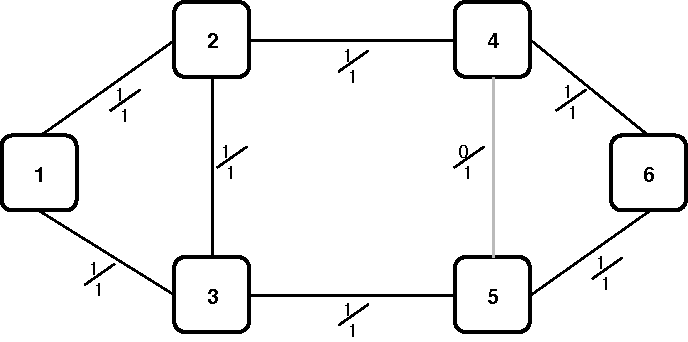
\includegraphics[width=12cm]{sdf/ilp/translucent_survivability/figures/physical_topology_high}
\caption{Translucent without survivability in high scenario: Physical topology after dimensioning.}
\label{physical3_high}
\end{figure}

\begin{figure}[h!]
\centering
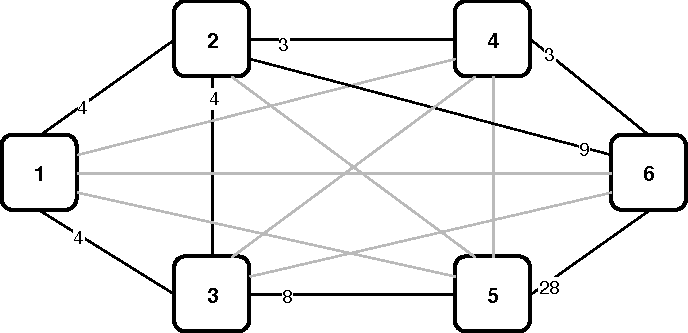
\includegraphics[width=12cm]{sdf/ilp/translucent_survivability/figures/optical_topology_high}
\caption{Translucent without survivability in high scenario: Optical topology after dimensioning.}
\label{optical3_high}
\end{figure}

In table \ref{link_transluc_surv_ref_high} we can see the number of optical channels calculated using \ref{Capex_Link} and \ref{ILPOpaque_CAPEX} and the number of amplifiers for each link calculated using \ref{Capex_amplifiers}.
In table \ref{node_transluc_surv_ref_high} we can see the resulting nodal degree at the physical layer, the number of line ports and add ports using \ref{OXC_poxc_transluc} the number of LR transponders using \ref{EXC_pexc2_transluc} and the number of tributary ports using \ref{EXC_pexc1_transluc}.
\newpage
\begin{table}[h!]
\centering
\begin{tabular}{|| c | c | c ||}
 \hline
 \multicolumn{3}{|| c ||}{Information regarding links} \\
 \hline
 \hline
 Bidirectional Link & Optical Channels & Amplifiers\\
 \hline
 Node 1 <-> Node 2 & 4 & 4 \\
 Node 1 <-> Node 3 & 4 & 6 \\
 Node 2 <-> Node 3 & 4 & 0 \\
 Node 2 <-> Node 4 & 12 & 6 \\
 Node 3 <-> Node 5 & 8 & 8 \\
 Node 4 <-> Node 5 & 0 & 0 \\
 Node 4 <-> Node 6 & 12 & 7 \\
 Node 5 <-> Node 6 & 28 & 3 \\
 \hline
\end{tabular}
\caption{Table with information regarding links for translucent mode without survivability in high scenario.}
\label{link_transluc_surv_ref_high}
\end{table}

\begin{table}[h!]
\centering
\begin{tabular}{|| c | c | c | c | c | c ||}
 \hline
 \multicolumn{6}{|| c ||}{Information regarding nodes} \\
 \hline
 \hline
 \multicolumn{2}{|| c |}{ } & \multicolumn{2}{ c |}{Electrical part} & \multicolumn{2}{ c ||}{Optical part} \\
 \hline
 Node & Resulting Nodal Degree & Tributary Ports & LR Transponders & Add Ports & Line Ports\\
 \hline
 1 & 2 & 580 & 8 & 8 & 8 \\
 2 & 3 & 460 & 20 & 20 & 20 \\
 3 & 3 & 360 & 16 & 16 & 16 \\
 4 & 2 & 400 & 6 & 6 & 24 \\
 5 & 2 & 480 & 36 & 36 & 36 \\
 6 & 2 & 440 & 40 & 40 & 40 \\
\hline
\end{tabular}
\caption{Table with information regarding nodes for translucent mode without survivability in high scenario.}
\label{node_transluc_surv_ref_high}
\end{table}

Through the information obtained previously on the nodes we can now create tables with detailed information about each node.

\begin{table}[h!]
\centering
\begin{tabular}{|| c | c | c ||}
 \hline
 \multicolumn{3}{|| c ||}{Detailed description of Node 1} \\
 \hline
 \hline
 Electrical part & Number of total demands & Bit rate \\
 \hline
\multirow{3}{*}{290 tributary ports} & 130 & ODU0 \\
 & 130 & ODU1 \\
 & 30 & ODU2 \\
 \hline
  & Node<--Optical Channels-->Node & Bit rate \\
 \hline
\multirow{2}{*}{8 LR Transponders} & 1  <---- 4 ---->  2 & \multirow{2}{*}{100 Gbits/s} \\
  & 1  <---- 4 ---->  3 & \\
 \hline
 \hline
 Optical part & Node<--Optical Channels-->Node & Bit rate \\
 \hline
 \multirow{2}{*}{8 add ports} & 1  <---- 4 ---->  2 & \multirow{4}{*}{100 Gbits/s} \\
  & 1  <---- 4 ---->  3 & \\ \cline{1-2}
 \multirow{2}{*}{8 line ports} & 1  <---- 4 ---->  2 & \\
  & 1  <---- 4 ---->  3 & \\
\hline
\end{tabular}
\caption{Translucent without survivability in high scenario: Detailed description of node 1. The number of demands is distributed to the various destination nodes, this distribution can be observed in section \ref{high_traffic_scenario}.}
\end{table}
\newpage
\begin{table}[h!]
\centering
\begin{tabular}{|| c | c | c ||}
 \hline
 \multicolumn{3}{|| c ||}{Detailed description of Node 2} \\
 \hline
 \hline
 Electrical part & Number of total demands & Bit rate \\ \hline
\multirow{5}{*}{230 tributary ports} & 110 & ODU0 \\
 & 70 & ODU1 \\
 & 20 & ODU2 \\
 & 20 & ODU3 \\
 & 10 & ODU4 \\
 \hline
  & Node<--Optical Channels-->Node & Bit rate \\
  \hline
\multirow{4}{*}{20 LR Transponders} & 2  <---- 4 ---->  1 & \multirow{4}{*}{100 Gbits/s} \\
  & 2  <---- 4 ---->  3 & \\
  & 2  <---- 3 ---->  4 & \\
  & 2  <---- 9 ---->  6 & \\
 \hline
 \hline
 Optical part & Node<--Optical Channels-->Node & Bit rate \\
 \hline
 \multirow{4}{*}{20 add ports} & 2  <---- 4 ---->  1 & \multirow{8}{*}{100 Gbits/s} \\
  & 2  <---- 4 ---->  3 & \\
  & 2  <---- 3 ---->  4 & \\
  & 2  <---- 9 ---->  6 & \\ \cline{1-2}
 \multirow{4}{*}{20 line ports} & 2  <---- 4 ---->  1 & \\
  & 2  <---- 4 ---->  3 & \\
  & 2  <---- 3 ---->  4 & \\
  & 2  <---- 9 ---->  6 & \\
\hline
\end{tabular}
\caption{Translucent without survivability in high scenario: Detailed description of node 2. The number of demands is distributed to the various destination nodes, this distribution can be observed in section \ref{high_traffic_scenario}.}
\end{table}

\begin{table}[h!]
\centering
\begin{tabular}{|| c | c | c ||}
 \hline
 \multicolumn{3}{|| c ||}{Detailed description of Node 3} \\
 \hline
 \hline
 Electrical part & Number of total demands & Bit rate \\
 \hline
 \multirow{4}{*}{180 tributary ports} & 70 & ODU0 \\
 & 60 & ODU1\\
 & 30 & ODU2\\
 & 20 & ODU3\\
 \hline
  & Node<--Optical Channels-->Node & Bit rate \\ \hline
 \multirow{3}{*}{16 LR Transponders} & 3  <---- 4 ---->  1 & \multirow{3}{*}{100 Gbits/s} \\
  & 3  <---- 4 ---->  2 & \\
  & 3  <---- 8 ---->  5 & \\
 \hline
 \hline
 Optical part & Node<--Optical Channels-->Node & Bit rate \\
 \hline
 \multirow{3}{*}{16 add ports} & 3  <---- 4 ---->  1 & \multirow{6}{*}{100 Gbits/s} \\
  & 3  <---- 4 ---->  2 & \\
  & 3  <---- 8 ---->  5 & \\ \cline{1-2}
 \multirow{3}{*}{16 line ports} & 3  <---- 4 ---->  1 & \\
  & 3  <---- 4 ---->  2 & \\
  & 3  <---- 8 ---->  5 & \\
\hline
\end{tabular}
\caption{Translucent without survivability in high scenario: Detailed description of node 3. The number of demands is distributed to the various destination nodes, this distribution can be observed in section \ref{high_traffic_scenario}.}
\end{table}

\newpage
\begin{table}[h!]
\centering
\begin{tabular}{|| c | c | c ||}
 \hline
 \multicolumn{3}{|| c ||}{Detailed description of Node 4} \\
 \hline
 \hline
 Electrical part & Number of total demands & Bit rate \\ \hline
\multirow{3}{*}{200 tributary ports} & 70 & ODU0 \\
 & 100 & ODU1 \\
 & 30 & ODU2 \\
 \hline
  & Node<--Optical Channels-->Node & Bit rate \\ \hline
 \multirow{2}{*}{6 LR Transponders} & 4  <---- 3 ---->  2 & \multirow{2}{*}{100 Gbits/s} \\
  & 4  <---- 3 ---->  6 & \\
 \hline
 \hline
 Optical part & Node<--Optical Channels-->Node & Bit rate \\
 \hline
 \multirow{2}{*}{6 add ports} & 4  <---- 3 ---->  2 & \multirow{5}{*}{100 Gbits/s} \\
  & 4  <---- 3 ---->  6 & \\ \cline{1-2}
 \multirow{3}{*}{24 line ports} & 4  <---- 3 ---->  2 & \\
  & 4  <---- 3 ---->  6 & \\
  & 2  <---- 9 ---->  6 & \\
\hline
\end{tabular}
\caption{Translucent without survivability in high scenario: Detailed description of node 4. The number of demands is distributed to the various destination nodes, this distribution can be observed in section \ref{high_traffic_scenario}.}
\end{table}

\begin{table}[h!]
\centering
\begin{tabular}{|| c | c | c ||}
 \hline
 \multicolumn{3}{|| c ||}{Detailed description of Node 5} \\
 \hline
 \hline
 Electrical part & Number of total demands & Bit rate \\ \hline
\multirow{5}{*}{240 tributary ports} & 140 & ODU0 \\
 & 40 & ODU1 \\
 & 40 & ODU2 \\
 & 10 & ODU3 \\
 & 10 & ODU4 \\
 \hline
  & Node<--Optical Channels-->Node & Bit rate \\ \hline
 \multirow{2}{*}{36 LR Transponders} & 5  <---- 8 ---->  3 & \multirow{2}{*}{100 Gbits/s} \\
  & 5  <---- 28 ---->  6 & \\
 \hline
 \hline
 Optical part & Node<--Optical Channels-->Node & Bit rate \\
 \hline
 \multirow{2}{*}{36 add ports} & 5  <---- 8 ---->  3 & \multirow{4}{*}{100 Gbits/s} \\
  & 5  <---- 28 ---->  6 & \\ \cline{1-2}
 \multirow{2}{*}{36 line ports} & 5  <---- 8 ---->  3 & \\
  & 5  <---- 28 ---->  6 & \\
\hline
\end{tabular}
\caption{Translucent without survivability in high scenario: Detailed description of node 5. The number of demands is distributed to the various destination nodes, this distribution can be observed in section \ref{high_traffic_scenario}.}
\end{table}

\newpage
\begin{table}[h!]
\centering
\begin{tabular}{|| c | c | c ||}
 \hline
 \multicolumn{3}{|| c ||}{Detailed description of Node 6} \\
 \hline
 \hline
 Electrical part & Number of total demands & Bit rate \\ \hline
\multirow{5}{*}{220 tributary ports} & 80 & ODU0 \\
 & 100 & ODU1 \\
 & 10 & ODU2 \\
 & 10 & ODU3 \\
 & 20 & ODU4 \\
 \hline
  & Node<--Optical Channels-->Node & Bit rate \\ \hline
 \multirow{3}{*}{40 LR Transponders} & 6  <---- 9 ---->  2 & \multirow{3}{*}{100 Gbits/s} \\
  & 6  <---- 9 ---->  4 & \\
  & 6  <---- 28 ---->  5 & \\
 \hline
 Optical part & Node<--Optical Channels-->Node & Bit rate \\
 \hline
 \multirow{3}{*}{40 add ports} & 6  <---- 9 ---->  2 & \multirow{6}{*}{100 Gbits/s} \\
  & 6  <---- 3 ---->  4 & \\
  & 6  <---- 28 ---->  5 & \\ \cline{1-2}
 \multirow{3}{*}{40 line ports} & 6  <---- 9 ---->  2 & \\
  & 6  <---- 3 ---->  4 & \\
  & 6  <---- 28 ---->  5 & \\
\hline
\end{tabular}
\caption{Translucent without survivability in high scenario: Detailed description of node 6. The number of demands is distributed to the various destination nodes, this distribution can be observed in section \ref{high_traffic_scenario}.}
\end{table}

In next page, we can see the routing information in table \ref{path_transluc_surv_ref_high}. These paths are bidirectional so the path from one node to another is the same path in the opposite direction.\\
Lastly through table \ref{scripttransluc_surv_ref_high} we can see the CAPEX result for this model. This value is obtained using equation \ref{ILPOpaque_CAPEX} and all of the constraints mentioned above.

\begin{table}[h!]
\centering
\begin{tabular}{|| c | c | c | c | c | c | c ||}
 \hline
 \multicolumn{7}{|| c ||}{CAPEX of the Network} \\
 \hline
 \hline
 \multicolumn{3}{|| c |}{ } & Quantity & Unit Price & Cost & Total \\
 \hline
 \multirow{3}{*}{Link Cost} & \multicolumn{2}{ c |}{OLTs} & 14 & 15 000 \euro & 210 000 \euro & \multirow{3}{*}{72 482 000 \euro} \\ \cline{2-6}
 & \multicolumn{2}{ c |}{100 Gbits/s Transceivers} & 144 & 5 000 \euro/Gbit/s & 72 000 000 \euro & \\ \cline{2-6}
 & \multicolumn{2}{ c |}{Amplifiers} & 68 & 4 000 \euro & 272 000 \euro & \\
 \hline
 \multirow{10}{*}{Node Cost} & \multirow{7}{*}{Electrical} & EXCs & 6 & 10 000 \euro & 60 000 \euro & \multirow{10}{*}{13 506 800 \euro} \\ \cline{3-6}
 & & ODU0 Ports & 1 200 & 10 \euro/port & 12 000 \euro & \\ \cline{3-6}
 & & ODU1 Ports & 1 000 & 15 \euro/port & 15 000 \euro & \\ \cline{3-6}
 & & ODU2 Ports & 320 & 30 \euro/port & 9 600 \euro & \\ \cline{3-6}
 & & ODU3 Ports & 120 & 60 \euro/port & 7 200 \euro & \\ \cline{3-6}
 & & ODU4 Ports & 80 & 100 \euro/port & 8 000 \euro & \\ \cline{3-6}
 & &Transponders& 126 & 100 000 \euro/port & 12 600 000 \euro & \\ \cline{2-6}
 & \multirow{3}{*}{Optical} & OXCs & 6 & 20 000 \euro & 120 000 \euro & \\ \cline{3-6}
 & & Line Ports & 144 & 2 500 \euro/port & 360 000 \euro & \\ \cline{3-6}
 & & Add Ports & 126 & 2 500 \euro/port & 315 000 \euro & \\
 \hline
 \multicolumn{6}{|| c |}{Total Network Cost} & 85 988 800 \euro \\
\hline
\end{tabular}
\caption{Translucent without survivability in high scenario: Detailed description of CAPEX for this scenario.}
\label{scripttransluc_surv_ref_high}
\end{table}

\newpage
\begin{table}[h!]
\centering
\begin{tabular}{|| c | c | c | c ||}
 \hline
 \multicolumn{4}{|| c ||}{Routing} \\
 \hline
 \hline
 o & d & Links & Demands \\
 \hline
 1 & 2 & \{(1,2)\} & 100 ODU0, 40 ODU1, 20 ODU2 \\ \hline
 1 & 3 & \{(1,3)\} & 20 ODU0, 80 ODU1, 20 ODU2 \\ \hline
 \multirow{2}{*}{1} & \multirow{2}{*}{4} & \{(1,2),(2,4)\} & 60 ODU0, 20 ODU1, 10 ODU2 \\
  & & \{(1,2),(2,4),(4,6),(6,4)\} & 20 ODU1, 10 ODU2 \\ \hline
 1 & 5 & \{(1,3),(3,5)\} & 20 ODU0 \\ \hline
 \multirow{2}{*}{1} & \multirow{2}{*}{6} & \{(1,2),(2,4),(4,6)\} & 60 ODU0, 80 ODU1 \\
  & & \{(1,3),(3,5),(5,6)\} & 20 ODU1 \\ \hline
 \multirow{2}{*}{2} & \multirow{2}{*}{3} & \{(2,1),(1,3)\} & 10 ODU3 \\
  & & \{(2,3)\} & 10 ODU3 \\ \hline
 2 & 4 & \{(2,4)\} & 20 ODU0, 60 ODU1 \\ \hline
 2 & 5 & \{(2,3),(3,5)\} & 100 ODU0, 20 ODU1, 20 ODU2 \\ \hline
 \multirow{3}{*}{2} & \multirow{3}{*}{6} & \{(2,4),(4,6)\} & 20 ODU1, 20 ODU3, 12 ODU4 \\
  & & \{(2,1),(1,3),(3,5),(5,6)\} & 4 ODU4 \\
  & & \{(2,3),(3,5),(5,6)\} & 4 ODU4\\ \hline
 \multirow{2}{*}{3} & \multirow{2}{*}{4} & \{(3,2),(2,4)\} & 20 ODU0, 20 ODU1 \\
  & & \{(3,5),(5,6),(6,4)\} & 20 ODU2 \\ \hline
 3 & 5 & \{(3,2),(2,4),(4,6),(6,4),(4,5)\} & 80 ODU0, 20 ODU1, 20 ODU2, 20 ODU3 \\ \hline
 3 & 6 & \{(3,2),(2,4),(4,6)\} & 20 ODU0 \\ \hline
 4 & 5 & \{(4,5)\} & 20 ODU0, 20 ODU1, 20 ODU2 \\ \hline
 4 & 6 & \{(4,6)\} & 20 ODU0, 60 ODU1\\ \hline
 5 & 6 & \{(5,4),(4,6)\} & 60 ODU0, 20 ODU1, 20 ODU2, 20 ODU4 \\
 \hline
\end{tabular}
\caption{Translucent without survivability in high scenario: Description of demands routing. In this case some demands follow different paths for the same pair of nodes.}
\label{path_transluc_surv_ref_high}
\end{table}

\subsection{Conclusions}

Once we have obtained the results for all the scenarios we will now draw some conclusions about these results. For a better analysis of the results will be created the table \ref{table_comparative_transluc_surv} with the number of line ports and add ports of the optical part, the tributary ports, the transponders and transceivers because they are important values for the cost of CAPEX, the cost of links, the cost of nodes and finally the cost of CAPEX.

\newpage
\begin{table}[h!]
\centering
\begin{tabular}{| c | c | c | c |}
 \hline
  & Low Traffic & Medium Traffic  & High Traffic \\
 \hline\hline
 Traffic (Gbit/s) & 500 & 5 000 & 10 000 \\ \hline
 Number of Add ports & 10 & 64 & 126 \\ \hline
 Number of Line ports & 12 & 72 & 144 \\ \hline
 Number of Tributary ports & 136 & 1 360 & 2 720 \\ \hline
 Number of Transceivers & 12 & 72 & 144 \\ \hline
 Number of Transponders & 10 & 64 & 126 \\ \hline
 Link Cost & 6 294 000 \euro & 36 482 000 \euro & 72 482 000 \euro \\ \hline
 Node Cost & 1 237 590 \euro & 6 945 900 \euro & 13 506 800 \euro \\ \hline
 CAPEX & \textbf{7 531 590 \euro} & \textbf{43 427 900 \euro} & \textbf{85 988 800 \euro} \\ \hline
 CAPEX/Gbit/s & \textbf{15 063 \euro/Gbit/s} & \textbf{8 686 \euro/Gbit/s} & \textbf{8 599 \euro/Gbit/s}\\
 \hline
\end{tabular}
\caption{Translucent without survivability: Table with the various CAPEX values obtained in the different traffic scenarios.}
\label{table_comparative_transluc_surv}
\end{table}

Looking at the previous table we can make some comparisons between the several scenarios:

\begin{itemize}
    \item Comparing the low traffic scenario with the others, we can see that, despite having an increase of factor ten (average scenario) and factor twenty (high scenario), the same increase does not occur in the final cost (it is lower). This happens because the number of transceivers is smaller than expected (an medium scenario of 120 would be expected and a high scenario would be expected in 240);
    \item Comparing the medium traffic scenario with the high traffic scenario, we can see that the factor increase is double and in the final cost this factor is very close but still lower;
    \item Comparing the cost with the traffic, we see that, for the low traffic scenario, the cost per traffic is very high in relation to the other two. We can conclude that a low traffic scenario becomes more expensive than a high traffic scenario.
\end{itemize}
